\documentclass[../../SperimentazioniPratiche.tex]{subfiles}

\begin{document}

% comandi necessari alla compilazione
\definecolor{cadmiumgreen}{rgb}{0.0, 0.42, 0.24}
\newcommand{\ok}{\textcolor{cadmiumgreen}{OK}} % Risultati quivalenti agli attesi
\newcommand{\ns}{\textcolor{red}{N.S.}} % non supportato
\newcommand{\nd}{\textcolor{red}{N.D.}} % non disponibile

% variabili dispositivi
\newcommand{\dispositivoA}{Moto G 2015}		
\newcommand{\dispositivoB}{Nexus 4}
\newcommand{\dispositivoC}{Galaxy S4 mini}

	\subsection{Prove effettuate}
	
		\subsubsection{Concretizzazione Prove}
			Ogni prova concettuale è effettuata attraverso una sua concretizzazione. Una concretizzazione rappresenta una prova reale effettuata sul campo, essa è identificata da un codice univoco:
			\begin{quote}
				\centering
				Prova \verb|[N][I].[T]|
			\end{quote}
			Dove:
			\begin{itemize}
				\item N è un carattere numerico che identifica la prova concettuale su cui la prova reale si basa;
				\item I è un carattere dell'alfabeto latino che identifica una impostazione dei valori delle variabili in input e output atteso della prova;
				\item T è un carattere numerico che identifica il numero di tentativo della prova.
			\end{itemize}
			
			Ogni prova reale è rappresentata all'interno di una \textbf{scheda} con le seguenti informazioni:
			\begin{itemize}
				\item Title: è il codice univoco che identifica la prova effettuata;
				\item Input: valori associati alle variabili in ingresso della prova. Se non richiesti è segnalato con 'N.R.';
				\item Output attesi: valori associati alle variabili in uscita dalla prova secondo gli input definiti in precedenza. Le variabili di output sono sempre identificate dalla variabile \verb|$RESULT| con un suffisso numerico se gli output siano più di uno;
				\item Output riscontrati: valori associati alle variabili in uscita dalla prova effettuata per ogni dispositivo elencato. 
				\begin{itemize}
					\item Se i risultati sono equivalenti ai risultati attesi, le variabili output sono marcate con \ok;
					\item Se non è possibile reperire i risultati perché l'applicazione non li supporta, le variabili output sono marcate con \ns;
					\item Se i risultati non corrispondono ai risultati attesi, vengono mostrate le informazioni errate in uscita dal dispositivo.
				\end{itemize}
			\end{itemize}
			
		%\subsubsection{Valori generali}
		
			
		\subsubsection{Registro prove}
		
			\begin{longtabu} {lcccc}
				\endhead
				\multicolumn{1}{l}{\textbf{Prova concettuale}} & \multicolumn{4}{c}{\textbf{Prove effettuate}}	\\
				\endhead
				\arrayrulecolor{gray}				
				
				\midrule
				\hyperref[subsec:Prova1]{Prova 1} & 
					\hyperref[2Prova1A.1]{1A.1} & 
					\hyperref[2Prova1A.2]{1A.2} & 
					\hyperref[2Prova1B.1]{1B.1} &
					\hyperref[2Prova1B.2]{1B.2} \\
					&
					\hyperref[2Prova1C.1]{1C.1} &
					\hyperref[2Prova1D.1]{1D.1} \\
					
				\midrule		
				\hyperref[subsec:Prova2]{Prova 2} &
					\hyperref[2Prova2A.1]{2A.1} &
					\hyperref[2Prova2B.1]{2B.1} &&\\
					
				\midrule
				\hyperref[subsec:Prova3]{Prova 3} &
					\hyperref[2Prova3A.1]{3A.1} &&&\\
					
				\midrule
				\hyperref[subsec:Prova4]{Prova 4} &
					\hyperref[2Prova4A.1]{4A.1} &&&\\
				

				\midrule					
				\hyperref[subsec:Prova5]{Prova 5} &
					\hyperref[2Prova5A.1]{5A.1} &&&\\
					
				\midrule
				\hyperref[subsec:Prova6]{Prova 6} &
					\hyperref[2Prova6A.1]{6A.1} &&&\\
					
				\midrule
				\hyperref[subsec:Prova7]{Prova 7} &
					\hyperref[2Prova7A.1]{7A.1} &&&\\
				
				\midrule
				\hyperref[subsec:Prova8]{Prova 8} &
					\hyperref[2Prova8A.1]{8A.1} &&&\\
				
				\midrule
				\hyperref[subsec:Prova9]{Prova 9} &
					\hyperref[2Prova9A.1]{9A.1} &&&\\
					
				\midrule
				\hyperref[subsec:Prova10]{Prova 10} &
					\hyperref[2Prova10A.1]{10A.1} &&&\\
					
				\midrule
				\hyperref[subsec:Prova11]{Prova 11} &
					\hyperref[2Prova11A.1]{11A.1} &&&\\
					
				\midrule
				\hyperref[subsec:Prova12]{Prova 12} &
					\hyperref[2Prova12A.1]{12A.1} &&&\\	
				
				\midrule
				\hyperref[subsec:Prova13]{Prova 13} &
					\hyperref[2Prova13A.1]{13A.1} &&&\\
					
				\midrule
				\hyperref[subsec:Prova14]{Prova 14} &
					\hyperref[2Prova14A.1]{14A.1} &&&\\
					
				\midrule
				\hyperref[subsec:Prova15]{Prova 15} &
					\hyperref[2Prova15A.1]{15A.1} &
					\hyperref[2Prova15B.1]{15B.1} &&\\
					
				\midrule
				\hyperref[subsec:Prova16]{Prova 16} &
					\hyperref[2Prova16A.1]{16A.1} &&&\\
				
				\arrayrulecolor{black}
				\bottomrule
				
				\caption{Sperimentazione 2016-05-26 - Registro prove effettuate}
			\end{longtabu}				
	
	\newpage		
		\subsubsection{Schede prove svolte}
			\paragraph*{}
			\label{2Prova1A.1}
			\begin{tcolorbox}[fonttitle=\bfseries, 
								adjusted title={\Large Prova 1A.1}, 
								breakable, 
								sharp corners=south,
								colback=white, 
								colframe=white!60!black]
								
				\begin{description}
				
					\item[Input] \ \par 
        				\begin{itemize}
        					\item \verb|$START| = Entrata torre B
        					\item \verb|$CAT| = Aule
							\item \verb|$END| = 1C150
        				\end{itemize}
        				
        			\tcbline 
        				
        			\item[Output atteso] \ \par
        				\begin{itemize}
        				
        					\item \verb|$RESULT1| = \{
        						1AD100, 1A150, 1BC45, 1BC50, 1C150
        					\}
        				
        					\item \verb|$RESULT2| = \{
        					\begin{enumerate}
        						\item Sali 1 piano di scale
								\item Apri la porta di fronte a te e svolta a sinistra
								\item Raggiungi la porta antincendio in fondo al corridoio
								\item destinazione raggiunta
        					\end{enumerate}
        					\}
        					
        				\end{itemize}

					\tcbline				
        				
        			\item[Output riscontrato] \ \par
        				\begin{description}
        				
        					\item[\dispositivoA] \ \par
        					\begin{itemize}
        						\item \verb|$RESULT1| = \ok
        						\item \verb|$RESULT2| = \ok
        					\end{itemize}      					
        					
        					\item[\dispositivoB] \ \par
        					\begin{itemize}
        						\item \verb|$RESULT1| = \ok
        						\item \verb|$RESULT2| = \ok
        					\end{itemize}
        					
        					\item[\dispositivoC] \ \par
        					\begin{itemize}
        						\item \verb|$RESULT1| = \ok
        						\item \verb|$RESULT2| = \ok
        					\end{itemize}
        					
        				\end{description}
        				
				\end{description}  
				
			\end{tcolorbox}
			
	
	\newpage
			\paragraph*{}
			\label{2Prova1B.1}		
			\begin{tcolorbox}[fonttitle=\bfseries, 
								adjusted title={\Large Prova 1B.1}, 
								breakable, 
								sharp corners=south,
								colback=white, 
								colframe=white!60!black]
								
				\begin{description}[leftmargin=0.7cm,labelwidth=!]
				
					\item[Input] \ \par 
        				\begin{itemize}
        					\item \verb|$START| = Entrata torre B
        					\item \verb|$CAT| = Toilette
							\item \verb|$END| = Toilette donne 1AD
        				\end{itemize}
        				
        			\tcbline 
        				
        			\item[Output atteso] \ \par
        				\begin{itemize}
							
							\item \verb|$RESULT1| = \{
								Toilette uomini 1BC, Toilette donne 1BC, Toilette uomini 1AB, Toilette uomini 1AB
							\}         				
        				
        					\item \verb|$RESULT2| = \{
        					\begin{enumerate}
        						\item Raggiungi entrata della Torre A
								\item Sali 1 piano di scale
								\item Apri la porta di fronte a te e svolta a destra
								\item destinazione raggiunta
        					\end{enumerate}
        					\}
        					       					
        					
        				\end{itemize}

					\tcbline        				
        				
        			\item[Output riscontrato] \ \par
        				\begin{description}
        				
        					\item[\dispositivoA] \ \par
        					\begin{itemize}
        						\item \verb|$RESULT1| = \ok
        						\item \verb|$RESULT2| = \ok
        					\end{itemize}      					
        					
        					\item[\dispositivoB] \ \par
        					\begin{itemize}
        						\item \verb|$RESULT1| = \ok
        						\item \verb|$RESULT2| = \ok
        					\end{itemize}
        					
        					\item[\dispositivoC] \ \par
        					\begin{itemize}
        						\item \verb|$RESULT1| = \ok
        						\item \verb|$RESULT2| = \ok
        					\end{itemize}
        					
        				\end{description}
        				
				\end{description}  
				
			\end{tcolorbox}



	
	\newpage
			\paragraph*{}
			\label{2Prova1B.2}
			\begin{tcolorbox}[fonttitle=\bfseries, 
								adjusted title={\Large Prova 1B.2}, 
								breakable, 
								sharp corners=south,
								colback=white, 
								colframe=white!60!black]
								
				\begin{description}[leftmargin=0.7cm,labelwidth=!]
				
					\item[Input] \ \par 
        				\begin{itemize}
        					\item \verb|$START| = Entrata torre B
							\item \verb|$CAT| = Toilette
							\item \verb|$END| = Toilette donne AD
        				\end{itemize}
        				
        			\tcbline 
        				
        			\item[Output atteso] \ \par
        				\begin{itemize}

							\item \verb|$RESULT1| = \{
								Toilette uomini 1BC, Toilette donne 1BC, Toilette uomini 1AB, Toilette uomini 1AB
							\}        				
        				
        					\item \verb|$RESULT2| = \{
        					\begin{enumerate}
        						\item Raggiungi entrata della Torre A
								\item Sali 1 piano di scale
								\item Apri la porta di fronte a te e svolta a destra
								\item destinazione raggiunta
        					\end{enumerate}
        					\}
        				\end{itemize}

					\tcbline        				
        				
        			\item[Output riscontrato] \ \par
        				\begin{description}
        				
        					\item[\dispositivoA] \ \par
        					\begin{itemize}
        						\item \verb|$RESULT1| = \ok
        						\item \verb|$RESULT2| = \ok
        					\end{itemize}      					
        					
        					\item[\dispositivoB] \ \par
        					\begin{itemize}
        						\item \verb|$RESULT1| = \ok
        						\item \verb|$RESULT2| = \ok
        					\end{itemize}
        					
        					\item[\dispositivoC] \ \par
        					\begin{itemize}
        						\item \verb|$RESULT1| = \ok
        						\item \verb|$RESULT2| = \ok
        					\end{itemize}
        					
        				\end{description}
        				
				\end{description}  
				
			\end{tcolorbox}

	
	\newpage
	\paragraph*{}
	\label{2Prova1C.1}
			
			\begin{tcolorbox}[fonttitle=\bfseries, 
								adjusted title={\Large Prova 1C.1}, 
								breakable, 
								sharp corners=south,
								colback=white, 
								colframe=white!60!black]
								
				\begin{description}%[leftmargin=0.7cm,labelwidth=!]
				
					\item[Input] \ \par 
        				\begin{itemize}
							\item \verb|$START| = 1AD100 (ROI = 01000) 
        					\item \verb|$CAT| = Aule
							\item \verb|$END| = 1BC45
        				\end{itemize}
        				
        			\tcbline 
        				
        			\item[Output atteso] \ \par
        				\begin{itemize}
        				
        					\item \verb|$RESULT1| = \{
        						1A150, 1C150, 1AD100, 1BC50, 1BC45
        					\}
        				
        					\item \verb|$RESULT2| = \{
        					\begin{enumerate}
        						\item Oltrepassa la porta antincendio più vicina , svolta a sinistra ed oltrepassa la seconda porta
        						\item Scendi 1 piano di scale
        						\item Raggiungi l'entrata della torre B
        						\item Sali 1 piano di scale
        						\item Apri la porta di fronte a te e svolta a sinistra
        						\item Raggiungi la porta antincendio in fondo al corridoio
        						\item destinazione raggiunta
        					\end{enumerate}
        					\}
        					
        				\end{itemize}

					\tcbline				
        				
        			\item[Output riscontrato] \ \par
        				\begin{description}
        				
        					\item[\dispositivoA] \ \par
        					\begin{itemize}
        						\item \verb|$RESULT1| = \ok
        						\item \verb|$RESULT2| = \ok
        					\end{itemize}      					
        					
        					\item[\dispositivoB] \ \par
        					\begin{itemize}
        						\item \verb|$RESULT1| = \ok
        						\item \verb|$RESULT2| = \ok
        					\end{itemize}
        					
        					\item[\dispositivoC] \ \par
        					\begin{itemize}
        						\item \verb|$RESULT1| = \ok
        						\item \verb|$RESULT2| = \ok
        					\end{itemize}
        					
        				\end{description}
        				
				\end{description}  
				
			\end{tcolorbox}
			
	\newpage
	\paragraph*{}
	\label{2Prova1C.2}
			
			\begin{tcolorbox}[fonttitle=\bfseries, 
								adjusted title={\Large Prova 1C.2}, 
								breakable, 
								sharp corners=south,
								colback=white, 
								colframe=white!60!black]
								
				\begin{description}%[leftmargin=0.7cm,labelwidth=!]
				
					\item[Input] \ \par 
        				\begin{itemize}
        					\item \verb|$CAT| = Aule
							\item \verb|$END| = 1BC45
							\item \verb|$START| = 1AD100 (Minor = 01000)
        				\end{itemize}
        				
        			\tcbline 
        				
        			\item[Output atteso] \ \par
        				\begin{itemize}
        				
        					\item \verb|$RESULT1| = \{
        						1A150, 1C150, 1AD100, 1BC50, 1BC45
        					\}
        				
        					\item \verb|$RESULT2| = \{
        					\begin{enumerate}
        						\item Oltrepassa la porta antincendio più vicina , svolta a sinistra ed oltrepassa la seconda porta
        						\item Scendi 1 piano di scale
        						\item Raggiungi l'entrata della torre B
        						\item Sali 1 piano di scale
        						\item Apri la porta di fronte a te e svolta a sinistra
        						\item Raggiungi la porta antincendio in fondo al corridoio
        						\item Destinazione raggiunta
        					\end{enumerate}
        					\}
        					
        				\end{itemize}

					\tcbline				
        				
        			\item[Output riscontrato] \ \par
        				\begin{description}
        				
        					\item[\dispositivoA] \ \par
        					\begin{itemize}
        						\item \verb|$RESULT1| = \ok
        						\item \verb|$RESULT2| = \ok
        					\end{itemize}      					
        					
        					\item[\dispositivoB] \ \par
        					\begin{itemize}
        						\item \verb|$RESULT1| = \ok
        						\item \verb|$RESULT2| = \ok
        					\end{itemize}
        					
        					\item[\dispositivoC] \ \par
        					\begin{itemize}
        						\item \verb|$RESULT1| = \ok
        						\item \verb|$RESULT2| = \ok
        					\end{itemize}
        					
        				\end{description}
        				
				\end{description}  
				
			\end{tcolorbox}

	\newpage
			\paragraph*{}
			\label{2Prova1D.1}
			\begin{tcolorbox}[fonttitle=\bfseries, 
								adjusted title={\Large Prova 1D.1}, 
								breakable, 
								sharp corners=south,
								colback=white, 
								colframe=white!60!black]
								
				\begin{description}%[leftmargin=0.7cm,labelwidth=!]
				
					\item[Input] \ \par 
        				\begin{itemize}
							\item \verb|$START| = 1BC45
        					\item \verb|$CAT| = Aule
							\item \verb|$END| = 1AD100
        				\end{itemize}
        				
        			\tcbline 
        				
        			\item[Output atteso] \ \par
        				\begin{itemize}
        				
        					\item \verb|$RESULT1| = \{
        						1AD100, 1A150, 1BC45, 1BC50, 1C150
        					\}
        				
        					\item \verb|$RESULT2| = \{
        					\begin{enumerate}
        						\item Oltrepassa la porta antincendio più vicina, svolta a sinistra ed oltrepassa la seconda porta
        						\item Scendi 1 piano di scale
        						\item Raggiungi l'entrata della torre D
        						\item Sali 1 piano di scale
        						\item Apri la porta di fronte a te e svolta a sinistra 
        						\item Destinazione raggiunta
        					\end{enumerate}
        					\}
        					
        				\end{itemize}

					\tcbline				
        				
        			\item[Output riscontrato] \ \par
        				\begin{description}
        				
        					\item[\dispositivoA] \ \par
        					\begin{itemize}
        						\item \verb|$RESULT1| = \ok
        						\item \verb|$RESULT2| = \ok
        					\end{itemize}      					
        					
        					\item[\dispositivoB] \ \par
        					\begin{itemize}
        						\item \verb|$RESULT1| = \ok
        						\item \verb|$RESULT2| = \ok
        					\end{itemize}
        					
        					\item[\dispositivoC] \ \par
        					\begin{itemize}
        						\item \verb|$RESULT1| = \ok
        						\item \verb|$RESULT2| = \ok
        					\end{itemize}
        					
        				\end{description}
        				
				\end{description}  
				
			\end{tcolorbox}

	
	\newpage
			\paragraph*{}	
			\label{2Prova2A.1}
			\begin{tcolorbox}[fonttitle=\bfseries, 
								adjusted title={\Large Prova 2A.1}, 
								breakable, 
								sharp corners=south,
								colback=white, 
								colframe=white!60!black]
								
				\begin{description}[leftmargin=0.7cm,labelwidth=!]
				
					\item[Input] \ \par 
        				\begin{itemize}
        					\item \verb|$START| = Entrata torre B
							\item \verb|$CAT| = Toilette
							\item \verb|$PREF| = Ascensore
        					\item \verb|$END| = 1C150
        				\end{itemize}
        				
        			\tcbline 
        				
        			\item[Output atteso] \ \par
        				\begin{itemize}
        					\item \verb|$RESULT| = \{
        						\begin{enumerate}
        							\item Prendi l'ascensore e sali 1 piano
									\item Raggiungi la porta antincendio in fondo al corridoio
									\item Destinazione raggiunta
        						\end{enumerate}
        					\}
        				\end{itemize}

					\tcbline        				
        				
        			\item[Output riscontrato] \ \par
        				\begin{description}
        				
        					\item[\dispositivoA] \ \par
        					\begin{itemize}
        						\item \verb|$RESULT| = \ok
        					\end{itemize}      					
        					
        					\item[\dispositivoB] \ \par
        					\begin{itemize}
        						\item \verb|$RESULT| = \ok
        					\end{itemize}
        					
        					\item[\dispositivoC] \ \par
        					\begin{itemize}
        						\item \verb|$RESULT| = \ok
        					\end{itemize}
        					
        				\end{description}
        				
				\end{description}  
				
			\end{tcolorbox}



	
	\newpage
			\paragraph*{}
			\label{2Prova2B.1}	
			\begin{tcolorbox}[fonttitle=\bfseries, 
								adjusted title={\Large Prova 2B.1}, 
								breakable, 
								sharp corners=south,
								colback=white, 
								colframe=white!60!black]
								
				\begin{description}[leftmargin=0.7cm,labelwidth=!]
				
					\item[Input] \ \par 
        				\begin{itemize}
        					\item \verb|$START| = Entrata torre B
							\item \verb|$CAT| = Toilette
							\item \verb|$PREF| = Ascensore
        					\item \verb|$END| = 1C150
        				\end{itemize}
        				
        			\tcbline 
        				
        			\item[Output atteso] \ \par
        				\begin{itemize}
        					\item \verb|$RESULT| = \{
        					\begin{enumerate}
        						\item Raggiungi entrata della Torre A
        						\item Prendi l'ascensore e sali 1 piano
        						\item Destinazione raggiunta
        					\end{enumerate}
        					\}
        				\end{itemize}

					\tcbline        				
        				
        			\item[Output riscontrato] \ \par
        				\begin{description}
        				
        					\item[\dispositivoA] \ \par
        					\begin{itemize}
        						\item \verb|$RESULT| = \ok
        					\end{itemize}      					
        					
        					\item[\dispositivoB] \ \par
        					\begin{itemize}
        						\item \verb|$RESULT| = \ok
        					\end{itemize}
        					
        					\item[\dispositivoC] \ \par
        					\begin{itemize}
        						\item \verb|$RESULT| = \ok
        					\end{itemize}
        					
        				\end{description}

				\end{description}  
				
			\end{tcolorbox}



	
	\newpage
			\paragraph*{}	
			\label{2Prova3A.1}	
			\begin{tcolorbox}[fonttitle=\bfseries, 
								adjusted title={\Large Prova 3A.1}, 
								breakable, 
								sharp corners=south,
								colback=white, 
								colframe=white!60!black]
								
				\begin{description}[leftmargin=0.7cm,labelwidth=!]
				
					\item[Input] \ \par 
        				\begin{itemize}
        					\item \verb|$START| = 1A150
							\item \verb|$CHANGE| = Entrata torre B
							\item \verb|$END| = 1C150
        				\end{itemize}
        				
        			\tcbline 
        				
        			\item[Output atteso] \ \par
        				\begin{itemize}
        					\item \verb|$RESULT| = \{
        					\begin{enumerate}
        						\item Apri la porta di fronte a te e svolta a sinistra
        						\item Raggiungi la porta antincendio in fondo al corridoio
        						\item Destinazione raggiunta
        					\end{enumerate}
        					\}
        					\item \verb|$RESULT2| = Visualizzato avviso errore
        				\end{itemize}

					\tcbline        				
        				
        			\item[Output riscontrato] \ \par
        				\begin{description}
        				
        					\item[\dispositivoA] \ \par
        					\begin{itemize}
        						\item \verb|$RESULT1| = \ok
        						\item \verb|$RESULT2| = \ok
        					\end{itemize}      					
        					
        					\item[\dispositivoB] \ \par
        					\begin{itemize}
        						\item \verb|$RESULT1| = \ok
        						\item \verb|$RESULT2| = \ok
        					\end{itemize}
        					
        					\item[\dispositivoC] \ \par
        					\begin{itemize}
        						\item \verb|$RESULT1| = \ok
        						\item \verb|$RESULT2| = \ok
        					\end{itemize}
        					
        				\end{description}
        				
				\end{description}  
				
			\end{tcolorbox}



	
	\newpage	
			\paragraph*{}	
			\label{2Prova4A.1}
			\begin{tcolorbox}[fonttitle=\bfseries, 
								adjusted title={\Large Prova 4A.1}, 
								breakable, 
								sharp corners=south,
								colback=white, 
								colframe=white!60!black]
								
				\begin{description}[leftmargin=0.7cm,labelwidth=!]
				
					\item[Input] \ \par 
        				\begin{itemize}
        					\item \verb|$START| = 1A150
							\item \verb|$INST| = Raggiungi la porta antincendio in fondo al corridoio
							\item \verb|$END| = 1C150
        				\end{itemize}
        				
        			\tcbline 
        				
        			\item[Output atteso] \ \par
        				\begin{itemize}
        					\item \verb|$RESULT1| = 
        					\url{http://bucketclips01.s3.amazonaws.com/images/172742.jpg}
        					\item \verb|$RESULT2| = 
        					\url{http://bucketclips01.s3.amazonaws.com/images/172759.jpg}
        					\item \verb|$RESULT3| = Raggiungi la porta antincendio in fondo al corridoio. Percorrendo il corridoio dovresti vedere alla tua sinistra in successione l'aula 1A150, poi delle finestre ed infine l'aula 1C150. Alla tua destra invece dovresti vedere la toilette delle donne di fronte all'aula 1A150, successivamente l'aula 1AD100 (che ha 3 ingressi) ed infine la toilette degli uomini di fronte l'aula 1C150.
        				\end{itemize}

					\tcbline        				
        				
        			\item[Output riscontrato] \ \par
        				\begin{description}
        				
        					\item[\dispositivoA] \ \par
        					\begin{itemize}
        						\item \verb|$RESULT1| = \ok
        						\item \verb|$RESULT2| = \ok
        						\item \verb|$RESULT3| = \ok
        					\end{itemize}      					
        					
        					\item[\dispositivoB] \ \par
        					\begin{itemize}
        						\item \verb|$RESULT1| = \ok
        						\item \verb|$RESULT2| = \ok
        						\item \verb|$RESULT3| = \ok
        					\end{itemize}
        					
        					\item[\dispositivoC] \ \par
        					\begin{itemize}
        						\item \verb|$RESULT1| = \ok
        						\item \verb|$RESULT2| = \ok
        						\item \verb|$RESULT3| = \ok
        					\end{itemize}
        					
        				\end{description}
        				
        				
				\end{description}  
				
			\end{tcolorbox}



	
	\newpage	
			\paragraph*{}
			\label{2Prova5A.1}	
			\begin{tcolorbox}[fonttitle=\bfseries, 
								adjusted title={\Large Prova 5A.1}, 
								breakable, 
								sharp corners=south,
								colback=white, 
								colframe=white!60!black]
								
				\begin{description}[leftmargin=0.7cm,labelwidth=!]
				
					\item[Input] \ \par 
        				\begin{itemize}
        					\item \verb|$START| = 1A150
        					\item \verb|$END| = 1C150
        				\end{itemize}
        				
        			\tcbline 
        				
        			\item[Output atteso] \ \par
        				\begin{itemize}
        					\item \verb|$RESULT| = Visualizzata schermata home dell'applicazione
        				\end{itemize}

					\tcbline        				
        				
        			\item[Output riscontrato] \ \par
        				\begin{description}
        				
        					\item[\dispositivoA] \ \par
        					\begin{itemize}
        						\item \verb|$RESULT| = \ok
        					\end{itemize}      					
        					
        					\item[\dispositivoB] \ \par
        					\begin{itemize}
        						\item \verb|$RESULT| = \ok
        					\end{itemize}
        					
        					\item[\dispositivoC] \ \par
        					\begin{itemize}
        						\item \verb|$RESULT| = \ok
        					\end{itemize}
        					
        				\end{description}
        			
        				
				\end{description}  
				
			\end{tcolorbox}



	
	\newpage	
			\paragraph*{}	
			\label{2Prova6A.1}
			\begin{tcolorbox}[fonttitle=\bfseries, 
								adjusted title={\Large Prova 6A.1}, 
								breakable, 
								sharp corners=south,
								colback=white, 
								colframe=white!60!black]
								
				\begin{description}[leftmargin=0.7cm,labelwidth=!]
				
					\item[Input] \ \par 
        				N.R.
        			\tcbline 
        				
        			\item[Output atteso] \ \par
        				\begin{itemize}
        					\item \verb|$RESULT| = Visualizzazione avviso mappa non aggiornata
        				\end{itemize}

					\tcbline        				
        				
        			\item[Output riscontrato] \ \par
        				\begin{description}
        				
        					\item[\dispositivoA] \ \par
        					\begin{itemize}
        						\item \verb|$RESULT| = \ok
        					\end{itemize}      					
        					
        					\item[\dispositivoB] \ \par
        					\begin{itemize}
        						\item \verb|$RESULT| = \ok
        					\end{itemize}
        					
        					\item[\dispositivoC] \ \par
        					\begin{itemize}
        						\item \verb|$RESULT| = \ok
        					\end{itemize}
        					
        				\end{description}
        				
				\end{description}  
				
			\end{tcolorbox}



	
	\newpage	
			\paragraph*{}	
			\label{2Prova7A.1}
			\begin{tcolorbox}[fonttitle=\bfseries, 
								adjusted title={\Large Prova 7A.1}, 
								breakable, 
								sharp corners=south,
								colback=white, 
								colframe=white!60!black]
								
				\begin{description}[leftmargin=0.7cm,labelwidth=!]
				
					\item[Input] \ \par 
        				N.R.
        				
        			\tcbline 
        				
        			\item[Output atteso] \ \par
        				\begin{itemize}
        					\item \verb|$RESULT| = Visualizzazione avviso che invita a scaricare mappa
        				\end{itemize}

					\tcbline        				
        				
        			\item[Output riscontrato] \ \par
        				\begin{description}
        				
        					\item[\dispositivoA] \ \par
        					\begin{itemize}
        						\item \verb|$RESULT| = \ok
        					\end{itemize}      					
        					
        					\item[\dispositivoB] \ \par
        					\begin{itemize}
        						\item \verb|$RESULT| = \ok
        					\end{itemize}
        					
        					\item[\dispositivoC] \ \par
        					\begin{itemize}
        						\item \verb|$RESULT| = \ok
        					\end{itemize}
        					
        				\end{description}
        				
				\end{description}  
				
			\end{tcolorbox}



	
	\newpage	
			\paragraph*{}	
			\label{2Prova8A.1}
			\begin{tcolorbox}[fonttitle=\bfseries, 
								adjusted title={\Large Prova 8A.1}, 
								breakable, 
								sharp corners=south,
								colback=white, 
								colframe=white!60!black]
								
				\begin{description}[leftmargin=0.7cm,labelwidth=!]
				
					\item[Input] \ \par 
        				N.R.
        				
        			\tcbline 
        				
        			\item[Output atteso] \ \par
        				\begin{itemize}
        					\item \verb|$RESULT1| = Visualizzazione invito accensione bluetooth
        					\item \verb|$RESULT2| = Visualizzazione invito accensione localizzazione
        				\end{itemize}

					\tcbline        				
        				
        			\item[Output riscontrato] \ \par
        				\begin{description}
        				
        					\item[\dispositivoA] \ \par
        					\begin{itemize}
        						\item \verb|$RESULT1| = \ok
        						\item \verb|$RESULT2| = \ok
        					\end{itemize}      					
        					
        					\item[\dispositivoB] \ \par
        					\begin{itemize}
        						\item \verb|$RESULT1| = \ok
        						\item \verb|$RESULT2| = \ok
        					\end{itemize}
        					
        					\item[\dispositivoC] \ \par
        					\begin{itemize}
        						\item \verb|$RESULT1| = \ok
        						\item \verb|$RESULT2| = \ok
        					\end{itemize}
        					
        				\end{description}
        				
				\end{description}  
				
			\end{tcolorbox}



	
	\newpage
			\paragraph*{}		
			\label{2Prova9A.1}
			\begin{tcolorbox}[fonttitle=\bfseries, 
								adjusted title={\Large Prova 9A.1}, 
								breakable, 
								sharp corners=south,
								colback=white, 
								colframe=white!60!black]
								
				\begin{description}[leftmargin=0.7cm,labelwidth=!]
				
					\item[Input] \ \par 
        				\begin{itemize}
        					\item \verb|$POS| = Entrata torre B
        				\end{itemize}
        				
        			\tcbline 
        				
        			\item[Output atteso] \ \par
        				\begin{itemize}
        					\item \verb|$RESULT| = \{
        					\begin{itemize}[label={}]
        						\item UUID = 19235dd2-574a-4702-a42e-caccac06e325,
								\item MAJOR = 666,
								\item MINOR = 1,
								\item RSSI = rilevato,
								\item BATTERY = rilevato,
								\item DISTANCE = rilevato,
								\item BEACONTYPE = rilevato,
								\item BLUETOOTHADDRESS = C7:45:5B:25:E1:D3
        					\end{itemize}
        					\}
        				\end{itemize}

					\tcbline        				
        				
        			\item[Output riscontrato] \ \par
        				\begin{description}
        				
        					\item[\dispositivoA] \ \par
        					\begin{itemize}
        						\item \verb|$RESULT| = \ok
        					\end{itemize}      					
        					
        					\item[\dispositivoB] \ \par
        					\begin{itemize}
        						\item \verb|$RESULT| = \ok
        					\end{itemize}
        					
        					\item[\dispositivoC] \ \par
        					\begin{itemize}
        						\item \verb|$RESULT1| = \ok
        						\item \verb|$RESULT2| = \ok
        					\end{itemize}
        					
        				\end{description}
        				
				\end{description}  
				
			\end{tcolorbox}


	
	\newpage	
			\paragraph*{}
			\label{2Prova10A.1}
			\begin{tcolorbox}[fonttitle=\bfseries, 
								adjusted title={\Large Prova 10A.1}, 
								breakable, 
								sharp corners=south,
								colback=white, 
								colframe=white!60!black]
								
				\begin{description}[leftmargin=0.7cm,labelwidth=!]
				
					\item[Input] \ \par 
        				\begin{itemize}
        					\item \verb|$AREA| = 1A150 (ROI = 01000)
        				\end{itemize}
        				
        			\tcbline 
        				
        			\item[Output atteso] \ \par
        				\begin{itemize}
        					\item \verb|$RESULT| = (l'area circolare può variare)
        					\begin{center}
        						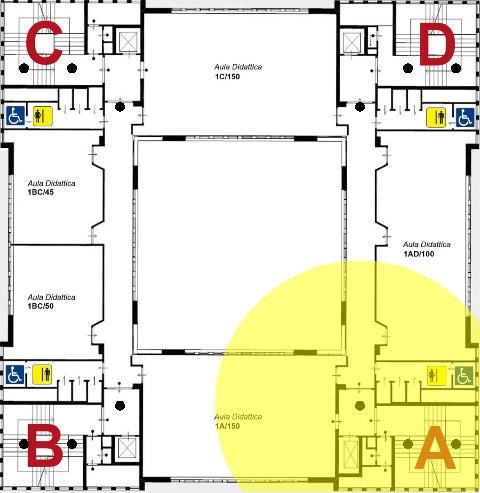
\includegraphics[scale=0.3]{img/ResultProva10A}
        					\end{center}
        				\end{itemize}

					\tcbline        				
        				
        			\item[Output riscontrato] \ \par
        				\begin{description}
        				
        					\item[\dispositivoA] \ \par
        					\begin{itemize}
        						\item \verb|$RESULT| = \ok
        					\end{itemize}      					
        					
        					\item[\dispositivoB] \ \par
        					\begin{itemize}
        						\item \verb|$RESULT| = \ok
        					\end{itemize}
        					
        					\item[\dispositivoC] \ \par
        					\begin{itemize}
        						\item \verb|$RESULT| = \ok
        					\end{itemize}
        					
        				\end{description}
        				
				\end{description}  
				
			\end{tcolorbox}



	
	\newpage		
			\paragraph*{}
			\label{2Prova11A.1}
			\begin{tcolorbox}[fonttitle=\bfseries, 
								adjusted title={\Large Prova 11A.1}, 
								breakable, 
								sharp corners=south,
								colback=white, 
								colframe=white!60!black]
								
				\begin{description}[leftmargin=0.7cm,labelwidth=!]
				
					\item[Input] \ \par 
        				\begin{itemize}
        					\item \verb|$START| = 1C150
							\item \verb|$WRONGSTRING| = qwerty
							\item \verb|$STRING| = Entrata 
							\item \verb|$END| = Entrata torre B
        				\end{itemize}
        				
        			\tcbline 
        				
        			\item[Output atteso] \ \par
        				\begin{itemize}
        					\item \verb|$RESULT1| = NULL
        					\item \verb|$RESULT2| = Visualizzato avviso \textit{Nessun risultato}
        					\item \verb|$RESULT3| = \{
        						Entrata torre A, Entrata torre B, Entrata torre C, Entrata torre D
        						\}
        					\item \verb|$RESULT4| = \{
								\begin{enumerate}
        									\item Oltrepassa la porta antincendio più vicina, svolta a sinistra ed oltrepassa la seconda porta
        									\item Scendi 1 piano di scale
        									\item Raggiungi l'entrata della torre B
        								\end{enumerate}							       
        						\}
        				\end{itemize}

					\tcbline        				
        				
        			\item[Output riscontrato] \ \par
        				\begin{description}
        				
        					\item[\dispositivoA] \ \par
        					\begin{itemize}
        						\item \verb|$RESULT1| = \ok
        						\item \verb|$RESULT2| = \ok
        						\item \verb|$RESULT3| = \ok
        						\item \verb|$RESULT4| = \ok
        					\end{itemize}      					
        					
        					\item[\dispositivoB] \ \par
        					\begin{itemize}
        						\item \verb|$RESULT1| = \ok
        						\item \verb|$RESULT2| = \ok
        						\item \verb|$RESULT3| = \ok
        						\item \verb|$RESULT4| = \ok
        					\end{itemize}
        					
        					\item[\dispositivoC] \ \par
        					\begin{itemize}
        						\item \verb|$RESULT1| = \ok
        						\item \verb|$RESULT2| = \ok
        						\item \verb|$RESULT3| = \ok
        						\item \verb|$RESULT4| = \ok
        					\end{itemize}
        					
        				\end{description}
        				
				\end{description}  
				
			\end{tcolorbox}


	
	\newpage		
			\paragraph*{}
			\label{2Prova12A.1}
			\begin{tcolorbox}[fonttitle=\bfseries, 
								adjusted title={\Large Prova 12A.1}, 
								breakable, 
								sharp corners=south,
								colback=white, 
								colframe=white!60!black]
								
				\begin{description}[leftmargin=0.7cm,labelwidth=!]
				
					\item[Input] \ \par 
        				\begin{itemize}
        					\item \verb|$SELECT| = 1C150
        				\end{itemize}
        				
        			\tcbline 
        				
        			\item[Output atteso] \ \par
        				\begin{itemize}
        					\item \verb|$RESULT1| = \{
        					\begin{itemize}
        						\item 1A150
								\item 1AD100
								\item 1BC45
								\item 1BC50
								\item 1C150
								\item Entrata torre A
								\item Entrata torre B
								\item Entrata torre C
								\item Entrata torre D
								\item Toilette donne 1AD
								\item Toilette donne 1BC
								\item Toilette uomini 1AD
								\item Toilette uomini 1BC
        					\end{itemize}
        					\}
        					\item \verb|$RESULT2| = \{
        						1\degree\ piano, Aule, Posti disponibili:45. 
        					\}
        				\end{itemize}

					\tcbline        				
        				
        			\item[Output riscontrato] \ \par
        				\begin{description}
        				
        					\item[\dispositivoA] \ \par
        					\begin{itemize}
        						\item \verb|$RESULT1| = \ok
        						\item \verb|$RESULT2| = \ok
        					\end{itemize}      					
        					
        					\item[\dispositivoB] \ \par
        					\begin{itemize}
        						\item \verb|$RESULT1| = \ok
        						\item \verb|$RESULT2| = \ok
        					\end{itemize}
        					
        					\item[\dispositivoC] \ \par
        					\begin{itemize}
        						\item \verb|$RESULT1| = \ok
        						\item \verb|$RESULT2| = \ok
        					\end{itemize}
        					
        				\end{description}
        				
				\end{description}  
				
			\end{tcolorbox}



	
	\newpage	
			\paragraph*{}	
			\label{2Prova13A.1}
			\begin{tcolorbox}[fonttitle=\bfseries, 
								adjusted title={\Large Prova 13A.1}, 
								breakable, 
								sharp corners=south,
								colback=white, 
								colframe=white!60!black]
								
				\begin{description}[leftmargin=0.7cm,labelwidth=!]
				
					\item[Input] \ \par 
        				\begin{itemize}
        					\item \verb|$POS| = Entrata torre C
        				\end{itemize}
        				
        			\tcbline 
        				
        			\item[Output atteso] \ \par
        				\begin{itemize}
        					\item \verb|$RESULT| = \{
        						Entrata torre C
        					\}
        				\end{itemize}

					\tcbline        				
        				
        			\item[Output riscontrato] \ \par
        				\begin{description}
        				
        					\item[\dispositivoA] \ \par
        					\begin{itemize}
        						\item \verb|$RESULT| = \ok
        					\end{itemize}      					
        					
        					\item[\dispositivoB] \ \par
        					\begin{itemize}
        						\item \verb|$RESULT| = \ok
        					\end{itemize}
        					
        					\item[\dispositivoC] \ \par
        					\begin{itemize}
        						\item \verb|$RESULT| = \ok
        					\end{itemize}
        					
        				\end{description}
        				
        			\tcbline
   
        				
				\end{description}  
				
			\end{tcolorbox}



	
	\newpage	
			\paragraph*{}
			\label{2Prova14A.1}	
			\begin{tcolorbox}[fonttitle=\bfseries, 
								adjusted title={\Large Prova 14A.1}, 
								breakable, 
								sharp corners=south,
								colback=white, 
								colframe=white!60!black]
								
				\begin{description}[leftmargin=0.7cm,labelwidth=!]
				
					\item[Input] \ \par 
        				\begin{itemize}
        					\item \verb|$START| = Entrata torre C
        					\item \verb|$END| = 1C150
							\item \verb|$INST| = Sali un piano di scale
        				\end{itemize}
        				
        			\tcbline 
        				
        			\item[Output atteso] \ \par
        				\begin{itemize}
        					\item \verb|$RESULT| = Visualizza avviso Connessione a Internet assente, impossibile scaricare la immagini
        				\end{itemize}

					\tcbline        				
        				
        			\item[Output riscontrato] \ \par
        				\begin{description}
        				
        					\item[\dispositivoA] \ \par
        					\begin{itemize}
        						\item \verb|$RESULT| = \ok
        					\end{itemize}      					
        					
        					\item[\dispositivoB] \ \par
        					\begin{itemize}
        						\item \verb|$RESULT| = \ok
        					\end{itemize}
        					
							\item[\dispositivoC] \ \par
        					\begin{itemize}
        						\item \verb|$RESULT| = \ok
        					\end{itemize}        					
        					
        				\end{description}
        				
				\end{description}  
				
			\end{tcolorbox}



	
	\newpage	
			\paragraph*{}
			\label{2Prova15A.1}	
			\begin{tcolorbox}[fonttitle=\bfseries, 
								adjusted title={\Large Prova 15A.1}, 
								breakable, 
								sharp corners=south,
								colback=white, 
								colframe=white!60!black]
								
				\begin{description}[leftmargin=0.7cm,labelwidth=!]
				
					\item[Input] \ \par 
        				\begin{itemize}
        					\item \verb|$START| = 1C150 (ROI = 1003)
        					\item \verb|$SPEED| = a passo lento
							\item \verb|$END| = Toilette donne 1BC
        				\end{itemize}
        				
        			\tcbline 
        				
        			\item[Output atteso] \ \par
        				\begin{itemize}
        					\item \verb|$RESULT| = Sali un piano di scale
        				\end{itemize}

					\tcbline        				
        				
        			\item[Output riscontrato] \ \par
        				\begin{description}
        				
        					\item[\dispositivoA] \ \par
        					\begin{itemize}
        						\item \verb|$RESULT| = \ok
        					\end{itemize}      					
        					
        					\item[\dispositivoB] \ \par
        					\begin{itemize}
        						\item \verb|$RESULT| = \ok
        					\end{itemize}
        					
        					\item[\dispositivoC] \ \par
        					\begin{itemize}
        						\item \verb|$RESULT| = \ok
        					\end{itemize}
        					
        				\end{description}
        				
        			\tcbline
        			
        			\item[Analisi risultati] \ \par
        				\begin{description}
        					\item[Considerazioni] \ \par
        						Nonostante la prova sia considerata accettabile, si segnala che non sempre il check dell'istruzione avviene nello stesso luogo in cui si trova l'utente. Con alcuni dispositivi avveniva prima con altri dopo. Tutto è molto aleatorio e dipende dal segnale emesso dai beacon.
        					
        					\item[Possibili miglioramenti] \ \par 
        						Aumentare la frequenza di aggiornamento dei beacon potrebbe essere una soluzione per incrementare l'affidabilità del check delle istruzioni.
        				\end{description}
        				
				\end{description}  
				
			\end{tcolorbox}



	
	\newpage		
			\paragraph*{}
			\label{2Prova15B.1}	
			\begin{tcolorbox}[fonttitle=\bfseries, 
								adjusted title={\Large Prova 15B.1}, 
								breakable, 
								sharp corners=south,
								colback=white, 
								colframe=white!60!black]
								
				\begin{description}[leftmargin=0.7cm,labelwidth=!]
				
					\item[Input] \ \par 
        				\begin{itemize}
        					\item \verb|$START| = 1C150
        					\item \verb|$SPEED| = a passo veloce
							\item \verb|$END| = Toilette donne 1BC
        				\end{itemize}
        				
        			\tcbline 
        				
        			\item[Output atteso] \ \par
        				\begin{itemize}
        					\item \verb|$RESULT| = Sali un piano di scale
        				\end{itemize}

					\tcbline        				
        				
        			\item[Output riscontrato] \ \par
        				\begin{description}
        				
        					\item[\dispositivoA] \ \par
        					\begin{itemize}
        						\item \verb|$RESULT| =\ok
        					\end{itemize}      					
        					
        					\item[\dispositivoB] \ \par
        					\begin{itemize}
        						\item \verb|$RESULT| = \ok
        					\end{itemize}
        					
        					\item[\dispositivoC] \ \par
        					\begin{itemize}
        						\item \verb|$RESULT| = \ok
        					\end{itemize}
        					
        				\end{description}
        				
					\tcbline
        			
        			\item[Analisi risultati] \ \par
        				\begin{description}
        					\item[Considerazioni] \ \par
        						Valgono le considerazioni descritte in precedenza.
        				\end{description}        				
        				
				\end{description}  
				
			\end{tcolorbox}



	
	\newpage		
			\paragraph*{}
			\label{2Prova16A.1}
			\begin{tcolorbox}[fonttitle=\bfseries, 
								adjusted title={\Large Prova 16A.1}, 
								breakable, 
								sharp corners=south,
								colback=white, 
								colframe=white!60!black]
				
				\begin{description}[leftmargin=0.7cm,labelwidth=!]
				
					\item[Input] \ \par 
        				\begin{itemize}
        					\item \verb|$START| = 1A150
							\item \verb|$NEXT| = 1C150
							\item \verb|$END| = Entrata torre D
        					\item \verb|$GRADE| = 180 gradi sessagesimali
        				\end{itemize}
        				
        			\tcbline 
        				
        			\item[Output atteso] \ \par
        				\begin{itemize}
        					\item \verb|$RESULT| = "Voltati"
        				\end{itemize}

					\tcbline        				
        				
        			\item[Output riscontrato] \ \par
        				\begin{description}
        				
        					\item[\dispositivoA] \ \par
        					\begin{itemize}
        						\item \verb|$RESULT| = \ok
        					\end{itemize}      					
        					
        					\item[\dispositivoB] \ \par
        					\begin{itemize}
        						\item \verb|$RESULT| = \ok
        					\end{itemize}
        					
        					\item[\dispositivoC] \ \par
        					\begin{itemize}
        						\item \verb|$RESULT| = \ok
        					\end{itemize}
        					
        				\end{description}
        				
        			\tcbline
        			
        			\item[Analisi risultati] \ \par
        				\begin{description}
        					\item[Considerazioni] \ \par
        						Nonostante la prova si consideri superata si segnala che l'accuratezza della bussola ricavata dai sensori del dispositivo varia enormemente dalla qualità hardware dello stesso, per cui alcune volte i dispositivi testati differivano seppur posizionati verso la stessa direzione. Altro fattore che influisce negativamente nella funzionalità sono le interferenze magnetiche esterne, anche il solo fatto di avere un dispositivo affiancato generava alterazioni sulle indicazioni. Si ritiene che allo stato attuale tale funzionalità non è da considerarsi completamente affidabile nonostante ciò però risulta di supporto alla funzionalità di navigazione.
        						
        					\item[Possibili miglioramenti] \ \par 
        						La variazione di performance risultata evidente nei dispositivi testati e le interferenze difficilmente prevedibili rende molto complesso il miglioramento di tale funzionalità. 
        				\end{description}

        				
				\end{description}  
				
			\end{tcolorbox}
			
			\newpage		
			\paragraph*{}
			\label{2Prova16B.1}
			\begin{tcolorbox}[fonttitle=\bfseries, 
								adjusted title={\Large Prova 16B.1}, 
								breakable, 
								sharp corners=south,
								colback=white, 
								colframe=white!60!black]
				
				\begin{description}[leftmargin=0.7cm,labelwidth=!]
				
					\item[Input] \ \par 
        				\begin{itemize}
        					\item \verb|$START| = 1A150
							\item \verb|$NEXT| = 1C150
							\item \verb|$END| = Entrata torre D
        					\item \verb|$GRADE| = 90 gradi sessagesimali
        				\end{itemize}
        				
        			\tcbline 
        				
        			\item[Output atteso] \ \par
        				\begin{itemize}
        					\item \verb|$RESULT| = "Ruota a sinistra"
        				\end{itemize}

					\tcbline        				
        				
        			\item[Output riscontrato] \ \par
        				\begin{description}
        				
        					\item[\dispositivoA] \ \par
        					\begin{itemize}
        						\item \verb|$RESULT| = \ok
        					\end{itemize}      					
        					
        					\item[\dispositivoB] \ \par
        					\begin{itemize}
        						\item \verb|$RESULT| = \ok
        					\end{itemize}
        					
        					\item[\dispositivoC] \ \par
        					\begin{itemize}
        						\item \verb|$RESULT| = \ok
        					\end{itemize}
        					
        				\end{description}
        				
        			\tcbline
        			
        			\item[Analisi risultati] \ \par
        				\begin{description}
        					\item[Considerazioni] \ \par
        						Valgono le considerazioni descritte in precedenza.
        				\end{description}
        				
				\end{description}  
				
			\end{tcolorbox}
	
	
\end{document}